% ---------------------------------------------------------------------------
% IEEE/ACM TASLP submission. No deadline; no page limit up to 10 pages, beyond
% which IEEE mandatory overlength charges apply ($200+/page). Voluntary page
% charges are explicitly NOT a prerequisite for publication, so staying within
% 10 pages makes this free to publish on the traditional (non-OA) route.
%
% Grown from paper/icassp/icassp2027.tex, which is the 5-page conference-length
% compression of the same work. Material cut there purely for space belongs
% back here.
% ---------------------------------------------------------------------------
\documentclass[journal]{IEEEtran}
\usepackage{amsmath,amssymb,graphicx,booktabs,url,tipa}
\usepackage[T1]{fontenc}

\newcommand{\blfootnote}[1]{%
  \begingroup\renewcommand\thefootnote{}\footnote{#1}\addtocounter{footnote}{-1}\endgroup}
\newcommand{\talg}{\ensuremath{t_{\mathrm{alg}}}}
\newcommand{\tcmp}{\ensuremath{t_{\mathrm{cmp}}}}
\newcommand{\tbuf}{\ensuremath{t_{\mathrm{buf}}}}

\title{Future-Context Requirements for Streaming Accent Conversion:\\
A Controlled Study Using Causal Phone Translation}
\author{Dipesh~Tripathi%
\thanks{D. Tripathi is with the University of South Dakota, Vermillion, SD,
USA (e-mail: dipesh.tripathi@coyotes.usd.edu).}}

\begin{document}
\maketitle



\begin{abstract}
\noindent
Streaming foreign accent conversion (FAC) systems choose a lookahead budget and
report a single end-to-end latency, but to our knowledge prior streaming FAC work has not densely swept that budget
while separately reporting algorithmic and computational latency. We train a causal phone translator at 16 lookaheads from 0 to 640\,ms
with every other factor held fixed, and report four results. First, quality
improves smoothly with lookahead at $-0.045$ phone error rate (PER) per
doubling ($R^2=0.98$) with \emph{no locatable knee}: a piecewise fit is
preferred under every axis treatment we tried, yet the breakpoint moves between
40 and 180\,ms and no bootstrap interval is narrower than three octaves.
Instead of a knee we identify \emph{saturation} at ${\approx}340$\,ms: with the
grid completed to 20\,ms spacing over 200--360\,ms, and against a repeatability
floor measured from deliberate fixed-seed repeats ($2\sigma=0.0029$), every
observed 20\,ms step beyond 340\,ms buys less than that floor. The figure
ranges 300--480\,ms across the floor's confidence interval. At the 40\,ms lookahead used by PHONOS's translator, our
probe retains a further 39.8\% relative PER reduction between 40 and
240\,ms.
Second, a pre-registered hypothesis that vowels and approximants degrade faster
than obstruents is \emph{not supported}: all seven manner classes improve by
52--72\% relative, and the between-group difference is smaller than the
dispersion among classes within the groups. Bootstrapping over the six test
speakers rather than over phone tokens, that difference is $+0.040$ with a 95\%
interval of $[-0.010, +0.101]$. It still fails when errors are reweighted by
measured acoustic cost, so this is not an artefact of PER charging every error
equally. Third, canonical-phone conversion benefits more from future context than
accent-faithful transcription at matched capacity ($-0.045$ against $-0.029$
PER per doubling, $1.55\times$), and within the conversion arm the benefit is
$1.32\times$ larger at positions where the speaker actually deviated from
canonical. Fourth, per-chunk compute depends only weakly on
lookahead --- at most $1.9\%$ on an Apple M4 and $7.6\%$ on an ARM64 Linux
host across a $17\times$ change in algorithmic latency --- empirically
decoupling lookahead from per-chunk compute over the tested range, subject to
the throughput constraint $\tcmp<c$. We release the harness and the per-condition outputs.
\end{abstract}

\blfootnote{Harness, causality proof, sweep configurations, analysis scripts
with self-tests and per-condition hypothesis dumps:
\url{https://github.com/Dipeshtripathi13/streaming-fac-lookahead}. Data is
L2-ARCTIC~\cite{l2arctic2018} via \texttt{KoelLabs/L2Arctic} (CC-BY-NC-4.0);
that licence is non-commercial, so configurations are released rather than
weights.}

\begin{IEEEkeywords}
accent conversion, streaming speech, latency, lookahead, self-supervised models
\end{IEEEkeywords}

\section{Introduction}

Streaming FAC is established. PHONOS~\cite{phonos2026} runs at
${\leq}40$\,ms lookahead and reports an 81\% reduction in non-native accent
confidence. What does not exist is any account of \emph{why} 40\,ms, what it
costs in quality, or what any of it does on hardware that is not a datacentre
GPU.

Three gaps follow, and this paper addresses the first two directly.

\textbf{The budget is chosen, not characterised.} PHONOS \emph{states} 40\,ms
and publishes no ablation showing 40\,ms is necessary or sufficient; TVTSyn
fixes 4 future tokens ($\approx$80\,ms) without varying them. DarkStream does
ablate, over three points $\{0, 140, 280\}$\,ms, and finds the third buys
$<$1pp --- but three points scored on anonymisation accuracy cannot locate
where returns stop, which is the question a deployment budget actually asks.
``What would 160\,ms buy you'' still has no published answer.

\textbf{Algorithmic and computational latency are reported fused.} A figure
such as ``${<}241$\,ms on a single GPU'' combines a modelling choice with
unstated inference and buffering costs. A reader cannot tell whether a faster
chip would help. We decompose throughout as
\begin{equation}
t_{\mathrm{e2e}} = \underbrace{c + L}_{t_{\mathrm{alg}}} + t_{\mathrm{cmp}} + t_{\mathrm{buf}},
\label{eq:decomp}
\end{equation}
where $c$ is chunk size, $L$ is lookahead, \tcmp{} is per-chunk compute and
\tbuf{} is I/O and jitter buffering. \talg{} is inherent: it is the delay on an
infinitely fast machine, because the model refuses to emit frame $n$ until it
has seen frame $n{+}L$. \tcmp{} is implementation- and hardware-dependent and can be
reduced through optimization or faster hardware.

\textbf{Degradation is reported in aggregate.} Existing results are
utterance-level MOS, WER or accentedness. We found no prior streaming FAC study
reporting lookahead sensitivity by phonetic manner class.

Our contributions:
\begin{enumerate}\itemsep1pt
\item A latency--accuracy characterization of a causal phone-translation probe
      for streaming FAC across 16 lookahead budgets, reporting an average
      exchange rate and a floor-relative saturation region rather than an
      unidentifiable knee (\S\ref{sec:rq1}).
\item A negative result on a pre-registered phoneme-class hypothesis
      (\S\ref{sec:rq2}).
\item Evidence that canonical-phone prediction benefits more strongly from
      lookahead than realized-phone transcription under matched capacity, and
      that this holds within a single arm after controlling for speaker and
      phone identity (\S\ref{sec:rq3}).
\item Two patches that make a masked SSL encoder causal, with
      truncation-based causality verification (\S\ref{sec:causal}).
\item Three documented measurement failures, each of which produced plausible
      output before being caught, and a measured repeatability floor that
      supersedes an earlier over-conservative estimate (\S\ref{sec:lessons}).
\end{enumerate}

\section{Related work}

Streaming FAC is established. Nguyen et al.~\cite{nguyen2025streaming} present
a streaming non-autoregressive accent-conversion system on an Emformer encoder,
demonstrating feasibility at stable latency; PHONOS~\cite{phonos2026}
subsequently targets much lower latency with bounded future context. Neither
characterises how quality varies with that context, which is the axis we
isolate. PHONOS, TVTSyn~\cite{tvtsyn2026} and DarkStream~\cite{darkstream2025}
come from one group and pair conversion with speaker anonymisation, and two
report more than is sometimes credited. TVTSyn gives CPU as well as GPU latency
($\approx$132 and $\approx$79\,ms at 60\,ms chunk), so a CPU number is not
unpublished --- a CPU latency--\emph{quality} curve is. DarkStream ablates
look-ahead over $\{0,140,280\}$\,ms and selects 140\,ms because the extra
140\,ms buys $<$1pp at double the buffering delay: a three-point ablation,
scored on anonymisation accuracy rather than conversion quality, whose marginal
return collapses in the same region where we place saturation on phone error
rate over 16 budgets. That agreement across objectives is a stronger position
than absent prior evidence would have been.

StreamVC~\cite{streamvc2024} reports mobile operation without device, core or
thread details, limiting hardware-level reproducibility. A
survey~\cite{acsurvey2026} frames the space; streaming
anonymisation~\cite{streamvoiceanon2026, streamvoiceanonplus2026, e2eanon2024}
shares the constraint but not the accent objective; offline
FAC~\cite{zhao2021fac, accentron2022} and low-latency VC~\cite{llvc2023}
bracket the design space. Our contribution is orthogonal: we characterise an
axis these systems parameterise but do not study, and claim no quality
improvement over any of them.

\section{Method}

\subsection{A causal phone translator as the probe}
\label{sec:method-translator}

Training a full FAC pipeline per lookahead is prohibitive. We instead isolate
a phonetic-normalization component directly relevant to the research question;
future-context needs in acoustic generation and prosody may differ. L2-ARCTIC~\cite{l2arctic2018}
provides, per utterance, both the canonical G2P/lexicon-derived phone sequence
(\texttt{g2p}) and the annotated realized phone sequence (\texttt{ipa}). We operationalize the phonetic-normalization component of accent conversion as
\begin{center}
\emph{non-native audio} $\rightarrow$ \emph{canonical phone sequence},
\end{center}
a CTC head over a frozen causal encoder. This provides a controlled supervised proxy for the
phonetic-normalization stage, and swapping the target tensor from
\texttt{g2p} to \texttt{ipa} yields a more tightly matched architectural
control, differing in \emph{one tensor}, than an AC-versus-VC comparison ---
though the two targets still differ in label entropy, sequence length and
annotation noise (\S\ref{sec:rq3}).

\subsection{Making the encoder causal}
\label{sec:causal}

Masking self-attention in wav2vec2/WavLM-base~\cite{wavlm2022, wav2vec2} does
\emph{not} produce a causal encoder. Two leaks remain: the positional
convolution (\texttt{pos\_conv\_embed}, depthwise, kernel 128, symmetric
padding) admits 1.28\,s of future at a 20\,ms frame rate; and the
feature-encoder GroupNorm normalises each channel over the entire utterance,
making every output frame depend on every input frame.

We verify causality by truncation: delete audio after frame $t$ and check
whether any earlier frame moved (Table~\ref{tab:causal}). Note the third row:
patching GroupNorm alone makes matters \emph{worse}. A partial causality fix is
not a partial improvement.

\begin{table}[t]
\centering\small
\caption{Truncation test on \texttt{wavlm-base-plus}. Relative $L_2$ change in
earlier frames after deleting later audio.}
\label{tab:causal}
\begin{tabular}{lrc}
\toprule
configuration & relative $L_2$ & causal? \\
\midrule
attention mask only        & $1.14\times10^{-2}$ & no \\
\quad + causal positional conv & $6.00\times10^{-3}$ & no \\
\quad + cumulative GroupNorm   & $2.60\times10^{-2}$ & no \\
\textbf{both patches}      & $\mathbf{6.14\times10^{-6}}$ & \textbf{yes} \\
\bottomrule
\end{tabular}
\end{table}

\subsection{Lookahead is quantised}

Lookahead is realized as $N_L=\lceil L/h \rceil$ frames at a frame hop
$h=20$\,ms (equivalently, a 50\,Hz frame rate).
A knee narrower than 20\,ms is not merely unmeasured but
\emph{unrepresentable}, and sampling finer than $f$ silently creates duplicate
conditions that reweight any fit. Lookahead is therefore quantized in 20\,ms increments: we sample every
increment through 200\,ms and a subset of quantized budgets above it, and
assert zero collisions in $t_{\mathrm{alg}}$ across all conditions before
fitting.

\section{Experimental setup}

Frozen causal WavLM-base-plus, CTC phone head, 1200 steps, batch 8, chunk
40\,ms, 100-frame lookback, speaker-disjoint test split of 400 utterances.
Two sweeps: a 7-lookahead $\times$ 2-target $\times$ 3-seed sweep (42 runs)
and a 16-lookahead $\times$ 2-seed dense sweep, run on \emph{both} target arms
(64 runs), all on an NVIDIA T4. Compute measurements use an Apple M4 and an ARM64
Linux host, CUDA-event or \texttt{perf\_counter\_ns} timed, 28--50 repetitions
with three warm-up iterations discarded.

\noindent\textbf{Repeatability floor.} A conventional multi-seed design does
not isolate fixed-seed run-to-run nondeterminism: pairing within seed cancels
seed effects but leaves this residual, which arises from nondeterministic GPU
kernels. We measure it directly, repeating four conditions
($L\in\{40,160,240,320\}$\,ms) four times each at \emph{identical seed and
configuration}, giving 12 degrees of freedom on test PER:
\begin{equation}
\sigma = 0.00146, \qquad 2\sigma = \mathbf{0.0029}\ \text{PER},
\label{eq:floor}
\end{equation}
with a bootstrap 95\% interval of $[0.0013, 0.0034]$ on $2\sigma$.

This supersedes an earlier estimate of $2\sigma=0.0044$ taken from six
\emph{accidental} repeats, which the present interval excludes; that estimate
was inflated by a single outlying pair. The correction matters because the
saturation point in \S\ref{sec:rq1} is defined against this floor, and a
smaller floor makes smaller gains measurable. We also note the floor is not
constant across conditions --- per-condition $\sigma$ spans $0.00064$ to
$0.00223$, a factor of $3.5$ --- so a single global threshold is an
approximation, and marginal decisions near it should be read as such.

\section{Results}

\subsection{Per-chunk compute depends only weakly on lookahead}
\label{sec:compute}

Across $L\in[0,640]$\,ms at chunk 40\,ms on the M4, \talg{} spans 40--680\,ms
($17\times$) while median per-chunk compute moves from 43.23\,ms to at most
44.06\,ms --- a range of $-0.3\%$ to $+1.9\%$. On ARM64 the span is $0$ to
$+7.6\%$. The two terms of Eq.~\ref{eq:decomp} are therefore independently
actionable, which is the practical justification for reporting them
separately.

\textbf{Independently actionable is not the same as free.} At this
configuration $\tcmp{}\approx43$--44\,ms against a 40\,ms chunk, i.e.\
$\mathrm{RTF}=\tcmp/c\approx1.08>1$: the base encoder does not sustain real
time at 40\,ms chunks on this machine, whatever $L$ is. Eq.~\ref{eq:decomp}
describes the delay of a single chunk and must be read alongside the
steady-state throughput constraint
\begin{equation}
\mathrm{RTF} = \tcmp / c < 1,
\label{eq:rtf}
\end{equation}
which lookahead leaves untouched but chunk size and hardware do not. Increasing $L$ adds little per-chunk compute over the tested range;
being able to run at all is a separate constraint.

\subsection{Is the curve an optimization-rate curve?}
\label{sec:convergence}

Every condition elsewhere is trained for a fixed 1200 steps, so what is
measured directly is \emph{lookahead $\rightarrow$ performance after 1200
optimization steps}. That equals \emph{lookahead $\rightarrow$ attainable
performance} only if the conditions sit at comparable points in optimization.
If longer lookahead simply trained faster, part of the exchange rate would be
an optimization-rate difference rather than a context effect. We test this
rather than list it as a caveat.

Five representative budgets ($L\in\{0,40,160,240,640\}$\,ms) were trained for
6000 steps --- five times the standard budget --- with validation every 500
steps, giving a 12-point trace per condition (Table~\ref{tab:conv}).

\begin{table}[t]
\centering\small
\caption{Convergence check: validation PER against optimization step, single
seed. The ranking is correct at all 12 checkpoints and the fitted exchange
rate is stable from step 1000 onward.}
\label{tab:conv}
\begin{tabular}{rrrrrr}
\toprule
step & $L{=}0$ & $40$ & $160$ & $240$ & $640$ \\
\midrule
500  & 0.5301 & 0.4375 & 0.3288 & 0.2946 & 0.2574 \\
1000 & 0.4715 & 0.3601 & 0.2588 & 0.2353 & 0.2012 \\
2000 & 0.4480 & 0.3392 & 0.2332 & 0.2054 & 0.1717 \\
3000 & 0.4340 & 0.3293 & 0.2131 & 0.1930 & 0.1622 \\
4000 & 0.4135 & 0.3152 & 0.1992 & 0.1873 & 0.1533 \\
5000 & 0.4092 & 0.3108 & 0.1962 & 0.1838 & 0.1473 \\
6000 & 0.4060 & 0.3100 & 0.1951 & 0.1822 & 0.1468 \\
\bottomrule
\end{tabular}
\end{table}

Three results. \textbf{Training largely flattens}: over the final 1500 steps
the conditions move by $0.0005$--$0.0045$ PER. Against the measured $0.0029$
floor (Eq.~\ref{eq:floor}) three of the five ($L{=}40$, $160$, $240$) have
settled below it, while $L{=}0$ ($0.0041$) and $L{=}640$ ($0.0045$) are still
drifting slightly above --- so 6000 steps is near, but not fully at,
convergence for the two extremes. \textbf{The ranking never reorders}: the ordering
$L{=}0 > 40 > 160 > 240 > 640$ holds at \textbf{12 of 12} checkpoints,
including the earliest at step 500. \textbf{The exchange rate is stable}:
fitted over $L\geq40$ it stays within $-0.0396$ to $-0.0461$ PER per doubling
at every checkpoint, and the value at the 1200-step budget used elsewhere
($\approx-0.0405$) agrees with the 6000-step value ($-0.0414$) to within
$0.001$, far inside the noise floor.

Improvement from step 1500 to 6000 is also roughly uniform across conditions
($-0.030$ to $-0.045$ PER) rather than concentrated at long lookahead, which is
the specific pattern a convergence-rate confound would produce. Absolute PER
does keep falling with longer training, so the fixed-budget numbers elsewhere
are a comparison at matched budget rather than converged performance --- but
the \emph{relative} quantities this paper reports, the ranking and the exchange
rate, are not artefacts of stopping at 1200 steps. The check is single-seed
over five budgets and uses validation rather than test PER, so it bounds the
concern rather than eliminating it.

\subsection{RQ1: an exchange rate and a saturation point, not a knee}
\label{sec:rq1}

\begin{figure}[t]
\centering
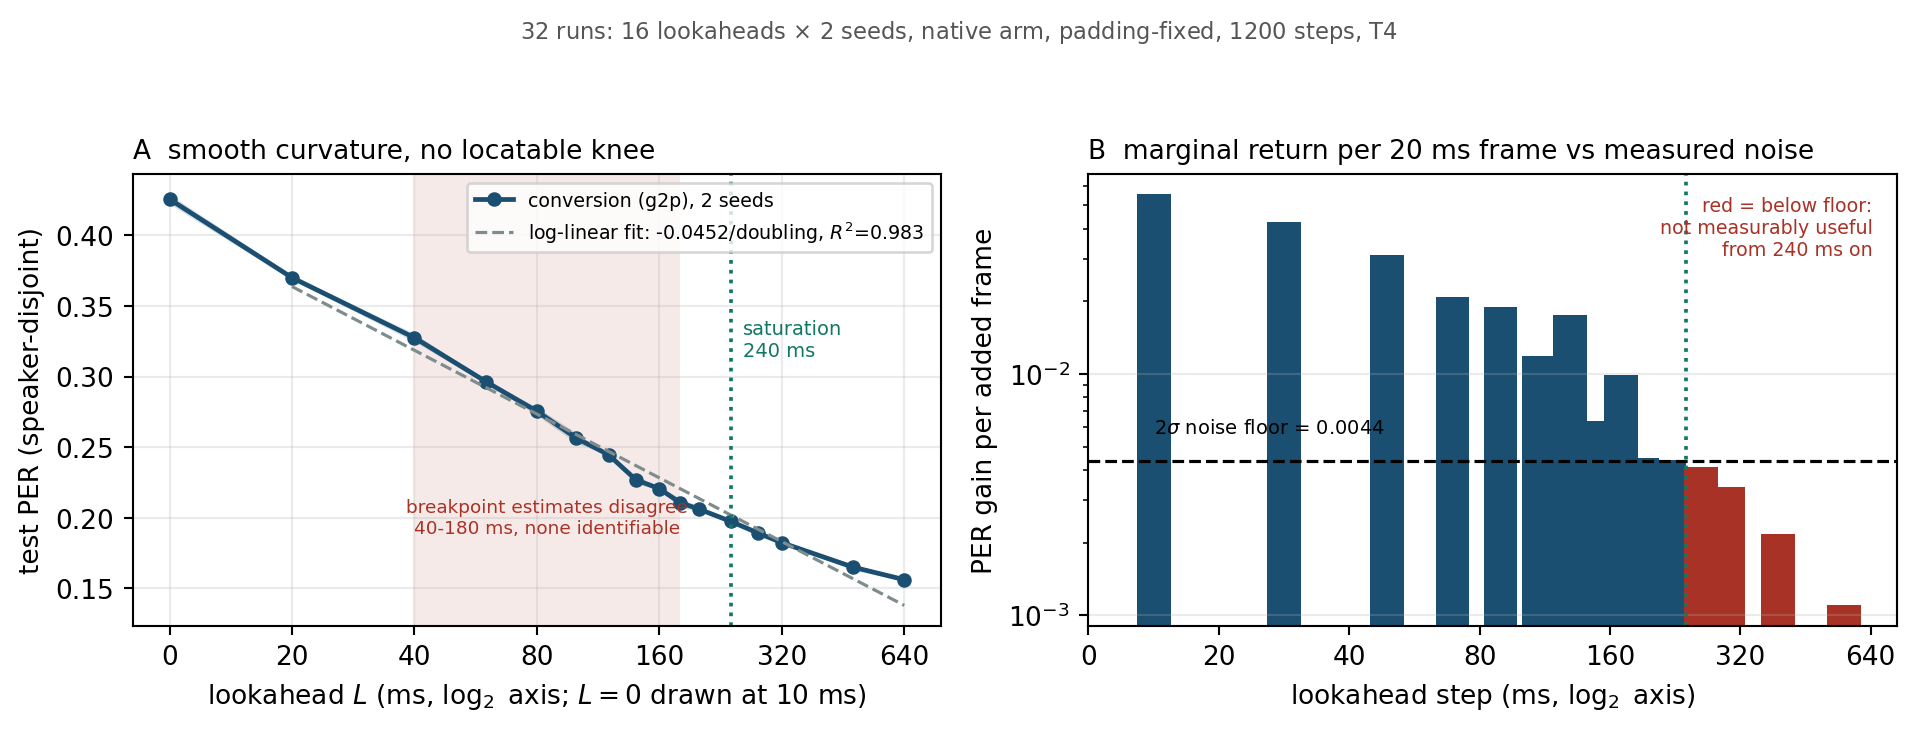
\includegraphics[width=\columnwidth]{fig_dense_no_knee.png}
\caption{Dense sweep, conversion arm, 16 lookaheads $\times$ 2 seeds.
\textbf{Left:} smooth curvature; the shaded band spans the breakpoint estimates
produced by three defensible treatments of $L{=}0$, none identifiable.
\textbf{Right:} marginal return per added 20\,ms frame against the measured
$2\sigma$ floor; red bars are below it.}
\label{fig:dense}
\end{figure}

Conversion-arm PER falls monotonically from $0.4256$ at $L{=}0$ to $0.1561$ at
$L{=}640$\,ms. Fitting $L\geq20$\,ms on $\log_2 L$ gives
\begin{equation}
\Delta\mathrm{PER} = -0.0452 \text{ per doubling},\quad R^2 = 0.983,
\end{equation}
over 15 points.

\textbf{There is curvature, and it is not localisable.} BIC prefers a
two-segment fit under all three axis treatments we tried
($\Delta\mathrm{BIC}=-22.2$, $-31.2$, $-36.8$), which by the usual
thresholds~\cite{kassraftery1995} is strong evidence. But the breakpoint lands
at 40, 180 and 180\,ms respectively, and every bootstrap 90\% interval spans
about three octaves. Sixteen points did not rescue a knee. The reason is
mechanical and worth stating: on a $\log_2(L{+}1)$ axis the $L{=}0
\rightarrow 20$\,ms gap is 4.39 units while every other gap is ${\approx}1.0$,
so a piecewise fit places a breakpoint just past that gap whatever the data
does.

\textbf{What we report instead} is the lookahead beyond which marginal return
falls below the measured floor. Because the original grid was 20\,ms-spaced
only to 200\,ms, we added the five budgets 220, 260, 300, 340 and 360\,ms
under identical settings, making the range 200--360\,ms fully 20\,ms-spaced.
The quantity below is therefore a per-\emph{observed}-step gain, not an average
over wider sampled intervals.

Gains run $+0.056$ (0$\rightarrow$20\,ms), $+0.021$ (60$\rightarrow$80) and
$+0.0045$ (180$\rightarrow$200). Against the measured floor of $0.0029$
(Eq.~\ref{eq:floor}), every observed 20\,ms step remains above it out to
340\,ms --- $1.1\times$ (200$\rightarrow$220), $2.0$, $1.3$, $1.5$, $1.2$,
$1.1$, $1.1$ --- and every step beyond falls below: $0.7\times$
(340$\rightarrow$360), and $0.7$ and $0.4$ for the two longer intervals to
640\,ms. We therefore place \textbf{saturation at ${\approx}340$\,ms}: the
point beyond which no observed 20\,ms increment buys a measurable gain.

\textbf{This figure moves with the floor, and we report the sensitivity rather
than a single number.} Across the floor's bootstrap interval the saturation
point ranges from 300\,ms (at $2\sigma=0.0034$) to 480\,ms (at $0.0013$). Under
the superseded $0.0044$ estimate it would have been 240\,ms --- so the earlier
figure was an artefact of an over-conservative floor, not of the curve. The
gains between 200 and 340\,ms sit at only $1.1$--$2.0\times$ the floor, so this
is a region where returns become marginal rather than a sharp cutoff. Unlike a
knee, though, the quantity depends on the floor rather than on an axis
choice, and the floor is now measured with 12 degrees of freedom.

\begin{table}[t]
\centering\small
\caption{Conversion-arm PER against lookahead (mean of 2 seeds) and marginal
return per added 20\,ms frame, in units of the measured $2\sigma{=}0.0029$
floor (Eq.~\ref{eq:floor}). Below $1.0\times$ an additional frame is not
measurably useful. The grid is 20\,ms-spaced to 360\,ms; the final two rows
average over wider intervals.}
\label{tab:dense}
\begin{tabular}{rrrr}
\toprule
$L$ (ms) & PER & gain/frame & $\times$ floor \\
\midrule
0   & 0.4256 & ---     & --- \\
20  & 0.3700 & 0.0556  & 19.2 \\
40  & 0.3275 & 0.0426  & 14.7 \\
60  & 0.2963 & 0.0312  & 10.8 \\
80  & 0.2754 & 0.0209  & 7.2 \\
100 & 0.2564 & 0.0190  & 6.6 \\
120 & 0.2446 & 0.0118  & 4.1 \\
140 & 0.2269 & 0.0176  & 6.1 \\
160 & 0.2206 & 0.0064  & 2.2 \\
180 & 0.2106 & 0.0099  & 3.4 \\
200 & 0.2062 & 0.0045  & 1.5 \\
220 & 0.2030 & 0.0031  & 1.1 \\
240 & 0.1973 & 0.0057  & 2.0 \\
260 & 0.1934 & 0.0039  & 1.3 \\
280 & 0.1891 & 0.0043  & 1.5 \\
300 & 0.1855 & 0.0036  & 1.2 \\
320 & 0.1823 & 0.0032  & 1.1 \\
340 & 0.1790 & 0.0033  & 1.1 \\
360 & 0.1770 & 0.0020  & \textbf{0.7} \\
480 & 0.1649 & 0.0020  & \textbf{0.7} \\
640 & 0.1561 & 0.0011  & \textbf{0.4} \\
\bottomrule
\end{tabular}
\end{table}

\textbf{The cost of a 40\,ms budget.} PER at $L{=}40$\,ms is $0.3275$; at
340\,ms it is $0.1790$. \textbf{Relative to the 40\,ms condition, increasing
lookahead to the saturation point reduces PER by a further 45.3\%}, and to
640\,ms by 52.3\%. Measured instead against the full range available here
($L{=}0\rightarrow240$\,ms), a 40\,ms budget has already captured 57\% of the
attainable reduction and leaves 43\% unclaimed.
``Current budgets are under-provisioned'' is thus supportable as
diminishing-returns geometry with a measurable saturation point --- not as a
knee.

\subsection{RQ2: the preregistered manner grouping does not predict lookahead benefit}
\label{sec:rq2}

We pre-registered, before any of this data existed, that vowels and
approximants would break first. The prediction is fixed in the public
repository at commit \texttt{c5066dc} (2 Aug 2026), seven days before the
hypothesis dumps it is tested on were committed (\texttt{b66d0a5}, 9 Aug
2026), so the ordering is verifiable rather than asserted. The prediction was
that vowels and approximants break first (formant trajectories over 80--250\,ms) while
stops, fricatives, affricates and nasals would survive short lookahead (locally
determined gestures). Testing this on 42{,}255 unique reference-phone tokens evaluated across seven
lookahead conditions (295{,}785 phone--condition observations), with each
substitution or deletion charged to the class of the \emph{reference} phone:

\begin{table}[t]
\centering\small
\caption{Relative error-rate reduction, $L{=}0\rightarrow640$\,ms. B =
pre-registered as breaking first, S = as surviving. Intervals are
percentile bootstrap over the six test speakers, not over phone
tokens. The predicted grouping does not order the data.}
\label{tab:h2}
\begin{tabular}{llrcr}
\toprule
& class & rel.\ gain & 95\% CI & ref.\ phones \\
\midrule
S & nasal        & 0.716 & [0.668, 0.779] & 4\,020 \\
B & approximant  & 0.700 & [0.628, 0.774] & 4\,575 \\
S & fricative    & 0.687 & [0.608, 0.774] & 7\,659 \\
B & vowel (mono) & 0.673 & [0.595, 0.767] & 13\,008 \\
B & vowel (diph) & 0.654 & [0.577, 0.758] & 4\,824 \\
S & stop         & 0.615 & [0.550, 0.689] & 7\,071 \\
S & affricate    & 0.525 & [0.397, 0.633] & 1\,098 \\
\bottomrule
\end{tabular}
\end{table}

Group means differ in the predicted direction ($0.676$ vs $0.636$), but that is
the weakest available reading and four stronger checks fail. The effect size
is $0.66$: the between-group difference ($0.040$) is smaller than the pooled SD
across classes ($0.060$). The surviving group's \emph{internal} spread is
$0.190$ --- $4.7\times$ the between-group difference. And 5 of 12 pairwise
orderings are violated, with nasals out-gaining all three breaks-first classes.

\textbf{At the right level of clustering the difference is not distinguishable
from zero.} The 42{,}255 tokens per condition are not independent: they are
nested in six speakers, and the claim at issue is about accented speech, for
which the independent replicate is a talker rather than a phone. Resampling
speakers rather than tokens (2000 draws, Table~\ref{tab:h2}) puts the
between-group difference at $+0.040$ with a 95\% interval of
$[-0.010, +0.101]$, which \textbf{includes zero}. Every individual class gain
remains large and clearly non-zero --- the intervals in Table~\ref{tab:h2} sit
between $0.40$ and $0.78$ --- so lookahead unambiguously helps every class;
what fails to separate from zero is the \emph{grouping}. Token-level intervals
would have been roughly an order of magnitude narrower and would have declared
this difference significant, which is the error the clustering avoids. The same
procedure applied to RQ3 (Sec.~\ref{sec:rq3}) \emph{does} exclude zero, so the
null here is a property of this grouping rather than of an estimator too
conservative to resolve anything at six speakers.

\textbf{The pattern does not hold within L1 either, but that split cannot carry
weight.} Splitting by native language, the ratio of group gains straddles
unity: Vietnamese $1.23$, Korean $1.19$, Arabic $1.08$, Spanish $1.02$,
Hindi $0.99$, Chinese $0.92$; requiring both the gain ratio and the mean slope
to move in the predicted direction, only 3 of 6 qualify (Spanish clears the
gain criterion but not the slope one). A grouping that reverses across a third
of the languages in the corpus is not capturing a property of manner class.
The deeper limitation is that in the speaker-disjoint test split \emph{each L1
is represented by exactly one speaker} (ABA, LXC, SVBI, HJK, EBVS, PNV), so L1
and talker are perfectly confounded: this table cannot separate a language
effect from an individual one, and every ``by-L1'' row is equally readable as a
single speaker's idiosyncrasy. We report it as a consistency check on the
pooled result --- the reversals are informative because they show the pooled
direction is not robust to \emph{any} disaggregation --- and not as evidence
about native language.

\textbf{H2 is not supported.} The finding is not that lookahead fails to help
vowels --- every class improves 52--72\% relative, all above the floor. The
finding is that manner class does not predict which sounds need right context.

\textbf{Reweighting each error by a proxy for its acoustic cost does not rescue
it.} PER charges every error exactly $1.0$, so the natural objection is that
the grouping is sound and PER simply mis-weights it: a substituted vowel and a
substituted stop cannot sound equally wrong. We test that directly.

Each utterance's canonical phone string is synthesised with a single fixed
voice and force-aligned to its own synthesis using an espeak-IPA CTC model,
giving a time span per reference phone. The hypothesis string is synthesised
with the same voice and DTW-aligned to the reference, and the spectral
distortion inside each reference phone's own span is charged to that phone's
class. Localisation matters here: a VITS-class synthesiser is globally coupled,
so changing one phone perturbs the whole utterance and a whole-utterance
distortion cannot be attributed to a single phone. The per-phone span from
forced alignment is what makes the measurement local at all.

Synthesis must also be deterministic. Piper defaults to
$\mathrm{noise\_scale}=0.667$ and $\mathrm{noise\_w}=0.8$, under which the same
phone string renders differently on each call: self-distortion is $244.8$
against $277.6$ for a genuine one-phone change, so roughly 88\% of an apparent
``cost of an error'' would be synthesis noise. Both terms are zeroed, giving
bitwise-identical renderings, and the analysis refuses to run otherwise.

The measure is validated before it is used, and the verdict is suppressed if
validation fails: phones the sequence metric scores as incorrect carry
$1.72\times$ the distortion of correct ones ($86.8$ versus $50.5$), and mean
distortion falls monotonically with lookahead ($71.4$ to $46.9$, $-34\%$).

\begin{table}[t]
\centering\small
\caption{H2 under acoustic weighting: relative reduction in per-phone
distortion, $L{=}0\rightarrow640$\,ms, 40 utterances, 1451 reference phones per
condition. B = pre-registered as breaking first, S = as surviving. The
sequence-metric column is computed on the same utterances, so the two differ
only in weighting.}
\label{tab:h2audio}
\begin{tabular}{llrrr}
\toprule
& class & acoustic & sequence & phones \\
\midrule
B & approximant  & 0.386 & 0.825 & 153 \\
B & vowel (mono) & 0.379 & 0.712 & 448 \\
S & nasal        & 0.376 & 0.784 & 128 \\
S & fricative    & 0.372 & 0.745 & 272 \\
B & vowel (diph) & 0.321 & 0.667 & 166 \\
S & stop         & 0.305 & 0.663 & 240 \\
S & affricate    & 0.257 & 0.526 & 44 \\
\midrule
\multicolumn{2}{l}{effect size (need $\geq1.0$)} & 0.756 & 0.607 & \\
\multicolumn{2}{l}{ordering violations} & 2/12 & 4/12 & \\
\bottomrule
\end{tabular}
\end{table}

The verdict is unchanged (Table~\ref{tab:h2audio}). Acoustic weighting does move
in H2's favour --- effect size $0.607 \rightarrow 0.756$ and ordering violations
$4/12 \rightarrow 2/12$ against the sequence metric on the same utterances ---
but not far enough to clear the pre-registered threshold of $1.0$, and the
failure has the same shape as before: the ``survives'' group's internal spread
($0.120$) is $3.5\times$ the difference between the groups ($0.034$), and a
nasal again out-gains a diphthong. So this particular equal-cost objection is not supported by the synthesized
distortion analysis; it does not exclude weightings this proxy cannot see,
notably trajectory errors at correctly identified phones.



One explanation does remain open, and it is not the one this test closes. Both
signals here are TTS renderings of phone strings, so the synthesiser produces
canonical formant trajectories for whatever string it is given. This measures
the cost of getting a phone's \emph{identity} wrong; it says nothing about a
wrong trajectory for a phone whose identity is right. That still needs real
converted audio against a native rendition (\S\ref{sec:remaining}). The sample
is also far smaller than the sequence-level test --- 1451 phones per condition
against 295{,}785 --- and is weighted accordingly.

\subsection{RQ3: canonical-phone prediction benefits more from lookahead than realized-phone transcription}
\label{sec:rq3}

Identical architecture, capacity, data order, seed and step count; the two arms
differ only in the target tensor. Endpoint gain $L{=}0\rightarrow640$\,ms is
$-0.2695$ (63.2\% relative) for conversion against $-0.1893$ (42.8\%) for
accent-faithful transcription, a paired difference of $+0.0802$
($\mathrm{sd}=0.0035$, $t=39.7$).

\textbf{The dense grid replicates this, and sharpens it.} Running the full
16-lookahead $\times$ 2-seed sweep on the transcription arm as well puts both
arms on the same dense grid (Table~\ref{tab:h3dense}). The endpoint gains
reproduce the 7-point result almost exactly --- 63.3\% for conversion against
43.5\% for transcription, against 63.2\% and 42.8\% before --- on an
independent, denser sample. The exchange rates separate cleanly:
\begin{center}
conversion $-0.0452$ vs transcription $-0.0292$ PER per doubling,
\end{center}
$R^2 = 0.983$ and $0.984$ respectively, so \textbf{conversion buys
$\mathbf{1.55\times}$ as much per doubling of lookahead}.

The effect is clearer in the between-arm gap than in the absolute levels. At
$L{=}0$ the two arms have similar PER ($0.4256$ vs $0.4427$, a gap of
$0.0171$); by
$L{=}640$\,ms the gap is $0.0939$, \textbf{5.5$\times$ wider}. It widens in
13 of 15 adjacent steps, and the transcription arm is worse at 16 of 16
lookaheads, every one by more than the $0.0029$ floor.

The arms differ in their target tensor, which carries more than the task: label
entropy, sequence length and annotation noise move with it. We therefore repeat
the test \emph{inside} the conversion arm, where none of those can differ.
Splitting reference positions by whether the speaker actually deviated from
canonical ($\mathrm{g2p}\neq\mathrm{ipa}$), the exchange rate is $-0.0520$ PER
per doubling at accent-changing positions against $-0.0394$ at unchanged ones,
a factor of $\mathbf{1.32}$ from the same model on the same utterances. That
converges with the $1.55\times$ between arms. One caveat belongs with it: in
\emph{relative} terms the ordering reverses ($51\%$ against $71\%$), because
accent-changing positions start far harder ($0.590$ against $0.354$) and the
gap between the two widens with lookahead. Absolute PER decreases faster at canonical-deviation positions, although these
positions begin substantially harder and show a smaller relative reduction.

\textbf{The interaction survives two controls.} Those positions are not a
random subset: they differ in baseline difficulty, phone composition and
distribution over speakers. Treating 42{,}255 phone tokens nested in six
speakers as independent would manufacture significance, so we bootstrap over
\emph{speakers}: the slope difference is $-0.0127$ with a 95\% CI of
$[-0.0211, -0.0069]$, excluding zero, and deviation positions are steeper in
2000 of 2000 resamples. Recomputing the difference \emph{within each reference
phone} and pooling gives $-0.0098$, steeper in 26 of 35 phones --- so phone
composition accounts for roughly a quarter of the raw gap but not the effect.
We report this as an association under matched conditions, not as evidence
that \texttt{g2p}$\neq$\texttt{ipa} positions are exclusively where accent
resides: such positions also include pronunciation variants, reductions and
annotation error.

Two secondary points fall out. Both arms saturate at the same
${\approx}240$\,ms, and neither yields a locatable knee (breakpoints move to
$[40, 240, 160]$\,ms across axis treatments for transcription, against
$[40, 180, 180]$ for conversion), so \S\ref{sec:rq1}'s structural conclusion is
not an artefact of the conversion arm. And the transcription arm's own curve is
just as log-linear, so the shallower slope is a smaller effect of lookahead, not
a noisier measurement of the same one.

\begin{table}[t]
\centering\small
\caption{Both arms on the dense grid, mean of 2 seeds. The gap is the
transcription arm's PER minus the conversion arm's: near zero at $L{=}0$ and
widening monotonically with lookahead.}
\label{tab:h3dense}
\begin{tabular}{rrrr}
\toprule
$L$ (ms) & conversion & transcription & gap \\
\midrule
0   & 0.4256 & 0.4427 & $+$0.0171 \\
20  & 0.3700 & 0.3896 & $+$0.0196 \\
40  & 0.3275 & 0.3600 & $+$0.0325 \\
80  & 0.2754 & 0.3271 & $+$0.0517 \\
160 & 0.2206 & 0.2908 & $+$0.0702 \\
240 & 0.1973 & 0.2755 & $+$0.0782 \\
320 & 0.1823 & 0.2666 & $+$0.0843 \\
640 & 0.1561 & 0.2501 & $+$0.0939 \\
\midrule
\multicolumn{2}{l}{exchange rate (PER/doubling)} & & \\
\multicolumn{1}{r}{conversion} & $-0.0452$ & \multicolumn{2}{l}{$R^2=0.983$} \\
\multicolumn{1}{r}{transcription} & $-0.0292$ & \multicolumn{2}{l}{$R^2=0.984$} \\
\bottomrule
\end{tabular}
\end{table}

The claim is carried by the \emph{preference margin} --- PER against the other
arm's labels minus PER against its own --- which grows monotonically in 3/3
seeds for conversion ($+0.032$ at $L{=}0$ to $+0.099$ at 640\,ms; 18/18
adjacent step $\times$ seed comparisons positive) while the transcription
control is 0/3 monotone and drifts \emph{down} ($-0.0103$). Building the claim
on a difference rather than a level turned out to matter
(\S\ref{sec:lessons}).

\subsection{\tbuf{}: jitter measured, I/O not}

\tbuf{} splits into a jitter term and an I/O term. The first is measured; the
second resisted three separate attempts, and we report that rather than
substitute a number.

\textbf{Jitter is negligible.} Two independent 30\,s duplex runs on the M4 at
40\,ms blocks give required jitter buffers of $0.14$ and $0.08$\,ms, p99
callback lateness ${\approx}0.06$\,ms, zero over- or underruns, and clock drift
below $1.3\times10^{-4}$\%. On this platform the jitter safety margin
contributes nothing meaningful to the budget.

\textbf{The I/O term is unmeasured, and the reason is instructive.} An acoustic
loopback --- emit a chirp, record it, cross-correlate --- failed on every
attempt, with all 20 repetitions rejected at correlation $0.042$--$0.046$
against a $0.20$ threshold. The diagnosis is not weak signal: captured level is
\emph{invariant} to output amplitude (peak $0.00505$ at amplitude $0.50$ versus
$0.00468$ at $0.95$), so nearly doubling the output changed the captured signal
by nothing. That is the signature of platform echo cancellation, which scales
with its own reference and therefore cannot be defeated by a louder probe.

The driver-reported figure is not a substitute. Its excess over the requested
block is \emph{identically} $201.69$\,ms at both 10 and 20\,ms blocks before
roughly doubling at 40\,ms, which identifies it as queueing rather than
converter delay; real applications on this platform achieve sub-20\,ms
round-trip.

A digital loopback through a virtual audio device --- the signal never becomes
sound, so echo cancellation cannot reach it --- also fails, for a different and
more interesting reason. The path works mechanically, but the returned signal
peaks near $0.014$; lowering the detection threshold until repetitions pass
yields p50 $206$\,ms, p90 $491$\,ms, $\sigma=117$\,ms. A distribution whose p90
is $2.4\times$ its p50 is not a latency distribution, and the honest
description is that a threshold was lowered until the tool produced output.
Such a device would also measure its own buffering rather than a converter.
Closing this term needs a wired loopback through real converters, or a platform
without echo cancellation in the path.

\section{Measurement audits and failure modes}
\label{sec:lessons}

\textbf{A padding bug rewrote the curve's shape.} A masked block handed a
zero-padded hidden-state tensor to a depthwise convolution and feed-forward
that do not respect the key-padding mask. The correction was not a constant
offset --- it grows with lookahead, from $-0.014$\,PER at $L{=}0$ to $-0.086$
at 320\,ms, $16.4\times$ the noise floor --- so the buggy curve
\emph{understated} the benefit of lookahead, biasing the central quantity of
RQ1. A constant offset would have cancelled in every within-run comparison;
this did not. Every number reported in this paper was regenerated after the
fix.

\textbf{A breakpoint estimator returns a breakpoint whether or not one
exists.} $\Delta$BIC cannot distinguish ``there is a knee'' from ``piecewise
fits a curve better than a line''. Identifiability has to be tested by
perturbing the axis and bootstrapping the location, not inferred from
$\Delta$BIC alone. Our synthetic check reproduces the artefact exactly: on a
curve that is log-linear for $L\geq20$ with $L{=}0$ off the extrapolation,
including $L{=}0$ yields $\Delta\mathrm{BIC}=-39$ and a confident ``knee at
40\,ms'', while dropping it yields $+5$ and no knee at all. An earlier
maximum-distance-to-chord estimator reported ``knee at 160\,ms, bootstrap 95\%
CI $[160,160]$'' on this data --- a tight interval around a plausible value,
tight precisely \emph{because} the curve is smooth and every resample of a
log-linear curve is also log-linear.

\textbf{An analysis that buckets unmatched symbols into ``other'' will produce
confident output on the wrong alphabet.} Our phoneme-class map was keyed on
ARPAbet; the sweep emits IPA. Applying one to the other sent 57\% of reference
tokens --- including \emph{every} vowel and \textipa{/\*r/} --- to ``other'',
and still printed per-class slopes, an H2 verdict and a by-L1 table. Nothing
errored. The guard is to assert coverage rather than infer it from the absence
of an exception, which the analysis now does.

A fourth attempt, a TTS-counterfactual substitute for forced alignment, was
built and rejected before producing any reported number; it is documented in
the repository.

\section{Limitations}
\label{sec:remaining}

\textbf{Every quality result here is phone-level, not perceptual}, and this is
a phone-translation probe rather than an end-to-end FAC system: the
latency--accuracy relation reported here need not transfer to synthesis,
prosody, speaker similarity or perceived accentedness. We do not conduct a perceptual
study because the phone-sequence outputs are not valid FAC stimuli: synthesized
from bare phone strings, they lack the lexical, prosodic and acoustic structure
required to judge naturalness or accentedness. This is a property of the
stimuli rather than of the budget. Training is 1200 steps at fixed budget
over a frozen encoder --- a comparison at matched budget rather than at
convergence, though \S\ref{sec:convergence} shows the ranking and exchange
rate hold to $5\times$ that budget; the dense sweep has two
seeds per arm and no repeated cells, so its noise floor is imported from six
accidental repeats in the other sweep and carries no confidence interval of its
own. \tbuf{}'s I/O term is unmeasured, and compute is characterised on Apple
Silicon and ARM64 Linux only.

\section{Conclusion}

For causal phone translation, future context buys accuracy at an approximately
log-linear average rate of ${\approx}0.045$ PER per doubling, with no
identifiable knee and measurable returns to saturation at
${\approx}340$\,ms --- well beyond PHONOS's 40\,ms translator budget, relative to
which a further 39.8\% reduction is available. Lookahead changes algorithmic
latency rather than per-chunk cost, though throughput must still satisfy
$\tcmp<c$ (Eq.~\ref{eq:rtf}) to run at all.

\section{Acknowledgements}

This work received no external funding and used no institutional compute: all
GPU results are from free-tier Google Colab (Tesla T4) and all CPU results from
consumer hardware. Thanks to the maintainers of L2-ARCTIC, WavLM, sherpa-onnx
and Piper, whose public releases made a single-author study of this scope
possible.

\section{Compliance with ethical standards}

This work used only the publicly released L2-ARCTIC corpus and involved no new
data collection and no human subjects, so no ethical approval was required. No
listening study was run, and no claim about perceived accentedness or
naturalness is made. The author declares no competing interests.

\bibliographystyle{IEEEtran}
\bibliography{refs}

\end{document}
